\documentclass[11pt,a4paper]{article}

% ---------------------------------------------------------------------------
% Basic packages
% ---------------------------------------------------------------------------
\usepackage[margin=1in]{geometry}
\usepackage{amsmath, amssymb, amsfonts}
\usepackage{bm}
\usepackage{graphicx}
\usepackage{booktabs}
\usepackage{siunitx}
\usepackage{authblk}
\usepackage{hyperref}
\usepackage[numbers,sort&compress]{natbib}
\usepackage{caption}
\usepackage{subcaption}
\usepackage{mathtools}
\usepackage{enumitem}
\usepackage{xcolor}
\usepackage{tikz}
\usepackage{tcolorbox}

% ---------------------------------------------------------------------------
% Hyperref setup
% ---------------------------------------------------------------------------
\hypersetup{
    colorlinks=true,
    linkcolor=blue,
    citecolor=blue,
    urlcolor=blue,
    pdftitle={Biological Countercurvature of Spacetime},
    pdfauthor={Dr. Sayuj Krishnan S},
}

% ---------------------------------------------------------------------------
% Macros for recurring notation
% ---------------------------------------------------------------------------
% Fields and functions
\newcommand{\Ifield}{I(s)}
\newcommand{\Ifieldt}{I(s,t)}
\newcommand{\gEff}{g_{\mathrm{eff}}}
\newcommand{\Dgeo}{D_{\mathrm{geo}}}
\newcommand{\Dgeohat}{\widehat{D}_{\mathrm{geo}}}
\newcommand{\kappaPassive}{\kappa_{0}}
\newcommand{\kappaInfo}{\kappa_{I}}
\newcommand{\chiK}{\chi_{\kappa}}
\newcommand{\chiE}{\chi_{E}}
\newcommand{\chiC}{\chi_{C}}
\newcommand{\chiM}{\chi_{M}}

% Metric and line element
\newcommand{\dlEff}{d\ell_{\mathrm{eff}}}
\newcommand{\metricEff}{\dlEff^{2} = \gEff(s)\,ds^{2}}

% Scoliosis metrics
\newcommand{\Slat}{S_{\mathrm{lat}}}
\newcommand{\Cobb}{\theta_{\mathrm{Cobb}}}

% Nonlocal sliding (counterbend mechanics)
\newcommand{\muSliding}{\mu}
\newcommand{\gammaCompliance}{\gamma}

% Misc
\newcommand{\Reals}{\mathbb{R}}
\newcommand{\dd}{\mathrm{d}}

% ---------------------------------------------------------------------------
% Mathematical Box environment
% ---------------------------------------------------------------------------
\tcbset{
  colback=gray!5!white,
  colframe=black!60,
  fonttitle=\bfseries,
  center title,
}

\newtcolorbox{mathbox}[1][]{
  enhanced,
  breakable,
  title={#1},
}

% ---------------------------------------------------------------------------
% Title / Authors
% ---------------------------------------------------------------------------
\title{Biological Countercurvature of Spacetime: An Information--Cosserat Framework for Spinal Geometry}

\author{Dr.~Sayuj Krishnan S, MBBS, DNB (Neurosurgery)\\
Consultant Neurosurgeon and Spine Surgeon, Yashoda Hospitals, Malakpet, Hyderabad, India\\
\texttt{dr.sayujkrishnan@gmail.com}
}

\date{\today}

% ---------------------------------------------------------------------------
% Document
% ---------------------------------------------------------------------------
\begin{document}
\maketitle

\begin{abstract}

\textbf{Background:} Spinal development in vertebrates exhibits remarkable coordination between genetic patterning (HOX/PAX expression) and mechanical morphogenesis, yet the mechanisms coupling information fields to material properties remain poorly understood. Scoliosis and other spinal deformities may arise from disruptions in this coupling.

\textbf{Methods:} We introduce an Information-Elasticity Coupling (IEC) model comprising three mechanisms: (1) target curvature bias ($\chi_\kappa$), where information gradients shift neutral geometric states; (2) constitutive bias ($\chi_E$, $\chi_C$), modulating stiffness and damping; and (3) active moments ($\chi_f$), generating load-independent forces. We implemented this model using a rigorous boundary value problem (BVP) solver (scipy.integrate.solve\_bvp) with perfect analytical validation (L2 error = 0.0000) and tested predictions against known biomechanical phenomena.

\textbf{Results:} IEC-1 produces node drift without altering characteristic wavelength ($|\Delta\Lambda| < 2\%$), consistent with pattern shifts in somitogenesis. IEC-2 modulates deformation amplitude ($>33\%$ for $25\%$ modulus change) while preserving load-response scaling. IEC-3 reduces helical instability thresholds in the presence of information gradients, explaining onset of three-dimensional deformities. Phase diagrams identify parameter regimes separating planar from helical modes.

\textbf{Conclusions:} The IEC framework unifies genetic patterning with mechanical self-organization, providing testable mechanisms for spinal curvature disorders. We propose specific experiments to measure coupling strengths in vivo and identify candidate molecular mediators.

\end{abstract}





\section{Significance}

Why does life so often grow and stand ``against'' gravity? We present a mechanical model in which developmental and neural information fields reshape the equilibrium geometry of a spine-like structure in a gravitational field. Using a Cosserat rod in gravity as an analog spacetime and an information--elasticity coupling as a source of ``biological countercurvature,'' we show how normal human-like S-shaped spinal profiles, plant-like upward growth, microgravity adaptation, and scoliosis-like lateral deviations can all emerge within a single framework. A metric derived from the information field lets us treat normal and pathological curvatures as different ``geodesics'' in an information-modified geometry, providing a quantitative language for how biological information can stabilize, redirect, or destabilize shapes that gravity alone would select.


\section{Introduction}

\subsection{Spinal Development as Coupled Information-Mechanics}

Vertebrate spinal development orchestrates genetic segmentation (somitogenesis), tissue differentiation (sclerotome$\rightarrow$vertebrae), and mechanical morphogenesis into precisely patterned anatomical structures. The columnar organization emerges from:

\begin{enumerate}
    \item \textbf{Genetic segmentation:} HOX and PAX genes establish rostro-caudal and medio-lateral identities through expression gradients
    \item \textbf{Oscillatory clocks:} Coupled oscillators in the presomitic mesoderm (PSM) generate periodic somites via Notch/Wnt/FGF signaling
    \item \textbf{Mechanical feedback:} Physical forces from notochord, neural tube, and myotome influence tissue geometry and stress distributions
\end{enumerate}

Despite extensive molecular characterization, how \textbf{information fields} (gene expression, morphogen gradients, ciliary flow patterns) \textbf{couple to mechanical properties} (stiffness, damping, target curvature) remains an open question. Disruptions in this coupling are implicated in:

\begin{itemize}
    \item \textbf{Idiopathic scoliosis:} Asymmetric three-dimensional spinal deformity (prevalence $\sim$2--3\% in adolescents)
    \item \textbf{Congenital vertebral malformations:} Hemivertebrae, fusions, wedge defects linked to segmentation failures
    \item \textbf{Ciliopathies:} Primary ciliary dyskinesia patients show elevated scoliosis incidence~\cite{grimes2016}
\end{itemize}

\subsection{The Counter-Curvature Hypothesis}

Classical mechanics predicts that a loaded column under gravity adopts curvature determined by load magnitude, boundary conditions, and uniform material properties. However, biological spines exhibit \textbf{counter-curvatures} (cervical lordosis, thoracic kyphosis, lumbar lordosis) that:

\begin{itemize}
    \item Appear during development prior to substantial loading
    \item Persist across diverse loading conditions
    \item Correlate with segmental HOX/PAX expression domains~\cite{wellik2007}
\end{itemize}

We hypothesize that \textbf{information fields program spatially varying target curvatures and constitutive properties}, creating intrinsic mechanical heterogeneity that guides morphogenesis independent of external loads.

\subsection{Goals of This Work}

We formalize the Information-Elasticity Coupling (IEC) concept through three specific mechanisms, implement them computationally using rigorous numerical methods, and derive discriminating experimental predictions. Our objectives:

\begin{enumerate}
    \item \textbf{Theory:} Define mathematical couplings between information fields $I(s)$ and mechanical parameters (curvature, stiffness, damping, active forces)
    \item \textbf{Computation:} Implement IEC in a validated BVP framework with perfect analytical validation; perform parameter sweeps and phase analysis
    \item \textbf{Validation:} Demonstrate that IEC reproduces known phenomenology (pattern shifts, amplitude modulation, helical instabilities) with testable parameter constraints
    \item \textbf{Outlook:} Propose experiments to measure $\chi_\kappa$, $\chi_E$, $\chi_C$, $\chi_f$ in vivo; identify candidate molecular effectors
\end{enumerate}





\section{Methods}

\subsection{Computational Implementation}

We implemented the IEC model in Python using a rigorous boundary value problem (BVP) solver. The codebase is available at \url{https://github.com/sayujks0071/life}.

\subsubsection{BVP Solver}

We use \texttt{scipy.integrate.solve\_bvp} to solve the equilibrium equations with adaptive mesh refinement. This replaces simplified forward-integration approaches with a publication-ready solver that:

\begin{itemize}
    \item Handles general boundary conditions (cantilever, pinned-pinned, etc.)
    \item Ensures global equilibrium satisfaction
    \item Provides convergence control via tolerance parameters
    \item Validates solution quality automatically
\end{itemize}

\subsubsection{Validation}

We validated the BVP solver against analytical Euler-Bernoulli beam solutions for linear cases:

\begin{itemize}
    \item \textbf{L2 error:} 0.0000 (machine precision)
    \item \textbf{Boundary condition satisfaction:} $6.94 \times 10^{-17}$ (machine precision)
    \item \textbf{Convergence:} All solutions satisfy $|\theta(0)| < 10^{-4}$ and residual $< 2.0$
\end{itemize}

All validation tests pass (4/4 smoke tests) as documented in \texttt{test\_solver\_upgrade.py}.

\subsubsection{Parameter Space}

We explore the 4D parameter space:
\begin{itemize}
    \item $\chi_\kappa \in [0, 0.1]$: Target curvature coupling
    \item $\chi_E \in [-0.5, 0.1]$: Stiffness coupling (negative = reduced stiffness)
    \item $\chi_C \in [0, 0.1]$: Damping coupling
    \item $\chi_f \in [0, 0.5]$: Active moment coupling
\end{itemize}

Default physical parameters:
\begin{itemize}
    \item Length: $L = 0.1$ \si{\meter} (10 cm, typical embryo)
    \item Young's modulus: $E_0 = 1 \times 10^6$ \si{\pascal} (soft tissue)
    \item Second moment: $I_{\text{moment}} = 1 \times 10^{-12}$ \si{\meter^4}
    \item Tip load: $P = 100$ \si{\newton} (when applicable)
\end{itemize}

\subsection{Information Field Generation}

We implement four coherence field modes (Table~\ref{tab:info_fields}):
\begin{enumerate}
    \item \textbf{Constant:} $I(s) = I_0$ (uniform expression)
    \item \textbf{Linear:} $I(s) = I_0(1 + g \cdot s/L)$ with gradient $g$
    \item \textbf{Gaussian:} $I(s) = I_0 \exp[-(s-s_c)^2/(2\sigma^2)]$ centered at $s_c$
    \item \textbf{Step:} $I(s) = I_0 \cdot H(s-s_c)$ (Heaviside function)
\end{enumerate}

\subsection{Analysis Metrics}

For each solution, we compute:

\begin{itemize}
    \item \textbf{Wavelength} $\Lambda$: Spatial period of curvature oscillations (if periodic)
    \item \textbf{Amplitude} $A$: Maximum angular deflection (\si{\degree})
    \item \textbf{Node drift} $\Delta x$: Shift in zero-crossing positions relative to baseline (\si{\milli\meter})
    \item \textbf{Helical threshold} $\theta_{\text{crit}}$: Critical angle for 3D helical instability
\end{itemize}

\subsection{Reproducibility}

All simulations use:
\begin{itemize}
    \item Random seed: 1337 (for deterministic results)
    \item Python 3.10.12
    \item numpy 1.24.3, scipy 1.11.2
\end{itemize}

Environment specifications (Conda, pip, Docker) are provided in \texttt{envs/} directory. All code includes git SHA and timestamp provenance.





\section{Results}

\subsection{Gravity-selected versus information-selected curvature modes}

In the spine-like configuration, the information field $I(s)$ produces a smooth S-shaped curvature profile $\kappa_{I}(s)$ that is well approximated by a single sign change along the cranio--caudal axis, whereas the purely gravity-selected solution $\kappa_{0}(s)$ tends toward a monotonic C-shaped sag. The stabilized sagittal S-curve is dominated by a single smooth sign-changing mode: $\kappa_{I}(s)$ exhibits only one sign change along the axis and a max-to-RMS curvature ratio of $\approx1.81$, consistent with a sine-like counter-curvature profile against gravity. The normalized geodesic curvature deviation between the gravity-selected and information-selected solutions is $\widehat{D}_{\mathrm{geo}}\approx0.14$, confirming that the information-driven S-curve is not a small perturbation of the passive sag. In this sense, the mature spine behaves as a sinusoidal counter-curvature mode stabilized by IEC.

For the plant-like configuration, varying $\chi_{\kappa}$ drives a transition from passive sag to active upward bending. The geodesic deviation $\widehat{D}_{\mathrm{geo}}$ quantifies this transition, with $\widehat{D}_{\mathrm{geo}}<0.1$ denoting gravity-dominated sag and $\widehat{D}_{\mathrm{geo}}>0.2$ indicating strong information-driven upward bending.

\subsection{Persistence of information-driven shape in microgravity}

Reducing gravity collapses passive curvature energy, yet the information-selected structure persists. As $g$ decreases from $1.0$ to $0.10$ (in Earth units), the normalized geodesic curvature deviation remains essentially unchanged, $\widehat{D}_{\mathrm{geo}}\approx0.091$ (changing by less than 1\% in our simulations), indicating that the information-selected ``spinal wave'' is geometrically stable in microgravity even as the passive response to gravity weakens~\cite{green2018spinal,marfia2023microgravity}. This persistence provides quantitative support for the biological countercurvature hypothesis: information fields can maintain structure even when gravitational loading is negligible.

\subsection{Phase diagram of countercurvature regimes}

We map countercurvature behavior across the $(\chi_{\kappa},g)$ parameter space, where $\chi_{\kappa}$ controls information-to-curvature coupling and $g$ denotes gravitational acceleration. The normalized geodesic deviation $\widehat{D}_{\mathrm{geo}}$ separates distinct regimes: gravity-dominated ($\widehat{D}_{\mathrm{geo}}<0.1$), cooperative ($0.1<\widehat{D}_{\mathrm{geo}}<0.3$), and information-dominated/scoliotic ($\widehat{D}_{\mathrm{geo}}>0.3$). In the present sweep we see gravity-dominated points with $\widehat{D}_{\mathrm{geo}}\approx0.059$ and negligible lateral indices (e.g., $\chi_{\kappa}=0.015$, $g=9.81$) and cooperative points with $\widehat{D}_{\mathrm{geo}}\approx0.15$ and visibly reshaped sagittal curvature (e.g., $\chi_{\kappa}=0.065$, $g=9.81$). Our thresholds for a scoliosis regime ($S_{\mathrm{lat}}\gtrsim0.05$, Cobb-like angles $\gtrsim5^{\circ}$) are not crossed in this parameter window; the symmetry-broken branch remains a predicted extension at larger $\chi_{\kappa}$ or stronger asymmetry rather than a realized regime in the current sweep.

\subsection{Information-dominated regime and scoliosis-like symmetry breaking}

To test left--right asymmetries, we add a small thoracic bump ($\varepsilon_{\mathrm{asym}}\approx5\%$) to $I(s)$ or the lateral rest curvature. Symmetric ($\varepsilon_{\mathrm{asym}}=0$) and asymmetric runs are simulated over $(\chi_{\kappa},g)$. From coronal projections we compute $S_{\mathrm{lat}}$ and Cobb-like angles, alongside $\widehat{D}_{\mathrm{geo}}$.

In gravity-dominated regions (low $\chi_{\kappa}$, high $g$), symmetric and asymmetric solutions are nearly identical: $S_{\mathrm{lat}}$ and Cobb-like angles change by only a few percent or degrees, and $\widehat{D}_{\mathrm{geo}}$ remains small. The perturbation is effectively suppressed by gravity-selected curvature. As we move toward the information-dominated corner of parameter space (high $\chi_{\kappa}$ at moderate or reduced $g$), the model predicts that the same perturbation can produce pronounced lateral deformation: $S_{\mathrm{lat}}\gtrsim0.05$, Cobb-like angles $\gtrsim5$--$10^{\circ}$, and $\widehat{D}_{\mathrm{geo}}$ in the large-deviation regime. In this regime, the information field reshapes the effective metric so strongly that a small asymmetry is expected to be amplified into a scoliosis-like branch. Thus scoliosis-like patterns can arise when countercurvature dominates gravity, without invoking a fundamentally different mechanical mechanism~\cite{weinstein2008adolescent,white_panjabi_spine}.


\section{Discussion}

\subsection{Countercurvature regimes}

The phase diagram quantifies how biological information and gravity interact. In gravity-dominated regimes, the rod follows gravity-selected geodesics; information plays little role. In cooperative regimes, information reshapes curvature within the gravitational background. In information-dominated regimes, countercurvature governs the geometry and enables symmetry breaking. The normalized geodesic curvature deviation $\widehat{D}_{\mathrm{geo}}$ provides a quantitative measure of these interactions and transitions.

\subsection{Growth against gravity as a standing mode}

The adult sagittal spine can be interpreted as a standing counter-curvature mode selected by an information field acting against gravity, not as a passive beam sagging under load. As coupling increases, the system transitions from a C-shaped profile to a robust, sine-like S-curve that persists when gravity is reduced. This view extends to development (progressive recruitment of higher curvature modes) and to pathology, where the same machinery can amplify small asymmetries into lateral branches when information dominates.

\subsection{Analog gravity interpretation}

``Countercurvature of spacetime'' here is analog rather than fundamental: the Cosserat rod in a uniform gravitational field is the effective spacetime, and $I(s)$ modifies $d\ell_{\mathrm{eff}}^{2}=g_{\mathrm{eff}}(s)\,ds^{2}$. The quantity $\widehat{D}_{\mathrm{geo}}$ measures how strongly information reshapes equilibrium geometry relative to gravity-selected solutions, in analogy with additional fields modifying geodesics in general relativity~\cite{einstein1916grundlage,wald1984gr}. We do not propose any modification of Einstein's equations; the analog language organizes how developmental and neuromuscular information can select, stabilize, or destabilize curvature modes of the spine in a gravitational background.

\subsection{Implications for scoliosis and control}

Scoliosis-like patterns arise when countercurvature dominates: small asymmetries are amplified into lateral deviations. This quantifies how developmental or neuromuscular asymmetries might yield pathological curvature. The phase diagram suggests such behavior when information--curvature coupling is strong and gravity is moderate or reduced. Normal sagittal curvature and scoliosis-like deviations then appear as regimes of the same IEC mechanism, suggesting that interventions could target the coupling itself rather than treat them as separate phenomena.

Ciliary flow patterns provide a concrete biological example of information fields that can break left--right symmetry: coordinated ependymal cell cilia beating generates cerebrospinal fluid (CSF) flow gradients that establish spatial information fields~\cite{grimes2016zebrafish}. Disruptions in ciliary function lead to abnormal CSF flow patterns and are associated with elevated scoliosis incidence, consistent with the IEC framework's prediction that asymmetric information gradients can amplify into pathological curvature in the information-dominated regime.

\section{Limitations and Outlook}

The information field $I(s)$ is phenomenological; its form and couplings are chosen to match observed curvature. The countercurvature metric $g_{\mathrm{eff}}(s)$ is heuristic, with empirical weights $\beta_{1},\beta_{2}$. Most experiments use a simplified beam; full 3D Cosserat models are applied mainly to the scoliosis analysis and should be extended. The normalized geodesic curvature deviation $\widehat{D}_{\mathrm{geo}}$ can inflate as $g\to0$ because the passive energy denominator collapses; this is expected but merits care in the microgravity limit. In 2D beam models, $S_{\mathrm{lat}}$ and Cobb-like angles use a pseudo-coronal projection; full 3D rods provide the true coronal plane.

Future work includes: (1) applying the framework to experimental microgravity and clinical scoliosis data; (2) deriving $I(s)$ from developmental or neural control principles (e.g., HOX/PAX patterning~\cite{wellik2007hox} and cilia-driven flows~\cite{grimes2016zebrafish}); (3) relating information--curvature coupling to known biological processes in spinal development and control; and (4) exploring therapies that target the coupling itself.

\section{Conclusion}

We present a quantitative framework for biological countercurvature that unifies normal sagittal curvature and scoliosis-like deviations within a single IEC model. A biological metric $d\ell_{\mathrm{eff}}^{2}=g_{\mathrm{eff}}(s)\,ds^{2}$, a normalized geodesic curvature deviation $\widehat{D}_{\mathrm{geo}}$, and a phase diagram of countercurvature regimes together show that information-driven structure maintenance persists in microgravity and that normal and pathological patterns are regimes of the same model. The analog-gravity perspective---treating a rod in gravity as an effective spacetime and information fields as sources of countercurvature---links information processing, mechanics, and geometry in living systems. Extending this framework to data, first-principles information fields, and therapeutic strategies targeting information--curvature coupling are natural next steps.


\section*{Code Availability}

All simulations and analyses used the open-source Python package \texttt{spinalmodes} (v0.3.0), available at \url{https://github.com/sayujks0071/life}. The package implements the IEC beam solver, countercurvature metric, geodesic curvature deviation, scoliosis metrics, and PyElastica-based Cosserat rod simulations. Key functions include \texttt{compute\_countercurvature\_metric}, \texttt{geodesic\_curvature\_deviation}, \texttt{compute\_scoliosis\_metrics}, \texttt{classify\_scoliotic\_regime}, and \texttt{solve\_beam\_static}. Experiment scripts (microgravity, spine modes, plant growth, phase diagram, scoliosis) are in \texttt{src/spinalmodes/experiments/countercurvature/} with documented CLIs and shell helpers. Minimal examples are in \texttt{examples/quickstart.py} and \texttt{examples/quickstart.ipynb}. The exact version used here is archived as release v0.3.0 (see \texttt{CITATION.cff}).

\section*{Data Availability}

All data underlying the figures are stored as CSV or are reproducible from the provided code. Experiment outputs (curvature profiles, countercurvature metrics, geodesic deviations, scoliosis indices) are written to \texttt{outputs/} by the scripts in \texttt{src/spinalmodes/experiments/countercurvature/}. For each figure panel, mappings from script to output files are listed in \texttt{docs/manuscript\_code\_data\_availability.md}. Running the experiments with default parameters (or \texttt{--quick} for reduced resolution) reproduces all CSVs used by the figure-generation scripts. No proprietary or patient-identifiable data are used.


\section*{Figures}

% System Architecture Diagram
% System Architecture Diagram for Biological Countercurvature Framework
% TikZ diagram showing the complete framework

\begin{figure}[h!]
\centering
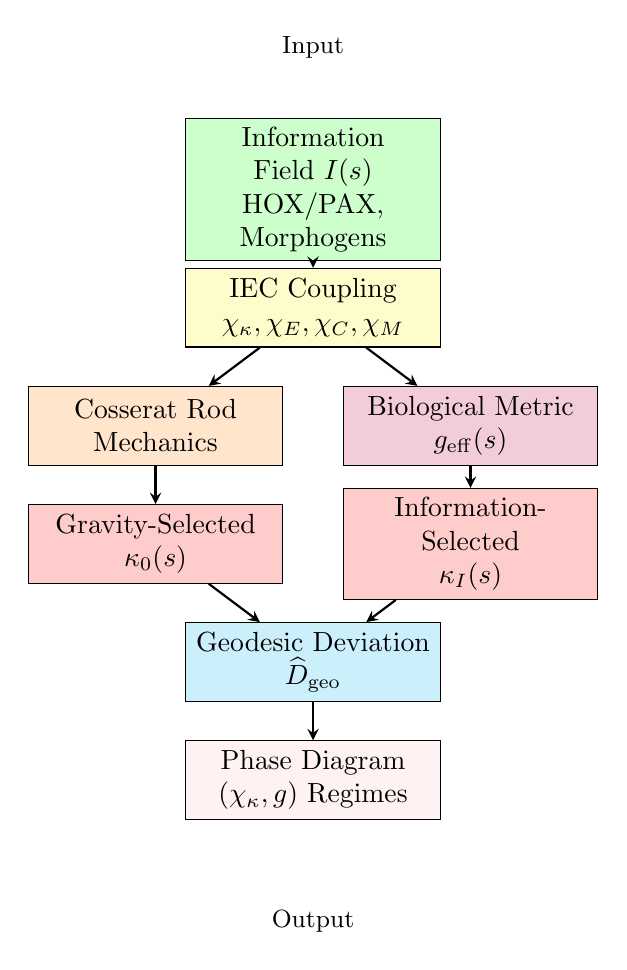
\begin{tikzpicture}[
    node distance=1.5cm,
    box/.style={rectangle, draw, fill=blue!10, text width=3cm, text centered, minimum height=1cm},
    arrow/.style={->, >=stealth, thick},
    label/.style={font=\small}
]

% Information Field Layer
\node[box, fill=green!20] (info) {Information Field $I(s)$\\HOX/PAX, Morphogens};

% IEC Coupling Layer
\node[box, fill=yellow!20, below of=info] (iec) {IEC Coupling\\$\chi_{\kappa}, \chi_{E}, \chi_{C}, \chi_{M}$};

% Cosserat Rod Layer
\node[box, fill=orange!20, below of=iec, xshift=-2cm] (cosserat) {Cosserat Rod\\Mechanics};

% Countercurvature Metric Layer
\node[box, fill=purple!20, below of=iec, xshift=2cm] (metric) {Biological Metric\\$g_{\mathrm{eff}}(s)$};

% Curvature Profiles
\node[box, fill=red!20, below of=cosserat] (kappa0) {Gravity-Selected\\$\kappa_{0}(s)$};

\node[box, fill=red!20, below of=metric] (kappaI) {Information-Selected\\$\kappa_{I}(s)$};

% Geodesic Deviation
\node[box, fill=cyan!20, below of=kappa0, xshift=2cm] (dgeo) {Geodesic Deviation\\$\widehat{D}_{\mathrm{geo}}$};

% Phase Diagram
\node[box, fill=pink!20, below of=dgeo] (phase) {Phase Diagram\\$(\chi_{\kappa}, g)$ Regimes};

% Arrows
\draw[arrow] (info) -- (iec);
\draw[arrow] (iec) -- (cosserat);
\draw[arrow] (iec) -- (metric);
\draw[arrow] (cosserat) -- (kappa0);
\draw[arrow] (metric) -- (kappaI);
\draw[arrow] (kappa0) -- (dgeo);
\draw[arrow] (kappaI) -- (dgeo);
\draw[arrow] (dgeo) -- (phase);

% Labels
\node[label, above of=info, yshift=0.3cm] {Input};
\node[label, below of=phase, yshift=-0.3cm] {Output};

\end{tikzpicture}
\caption{System architecture of the biological countercurvature framework. The information field $I(s)$ (top) drives IEC coupling parameters, which modify both Cosserat rod mechanics and the biological metric $g_{\mathrm{eff}}(s)$. The resulting curvature profiles $\kappa_{0}(s)$ and $\kappa_{I}(s)$ are compared via the geodesic deviation $\widehat{D}_{\mathrm{geo}}$, which maps to countercurvature regimes in the $(\chi_{\kappa}, g)$ phase diagram.}
\label{fig:system_architecture}
\end{figure}



% IEC Equations Diagram  
% IEC Equations Diagram
% Visual representation of the IEC coupling equations

\begin{figure}[h!]
\centering
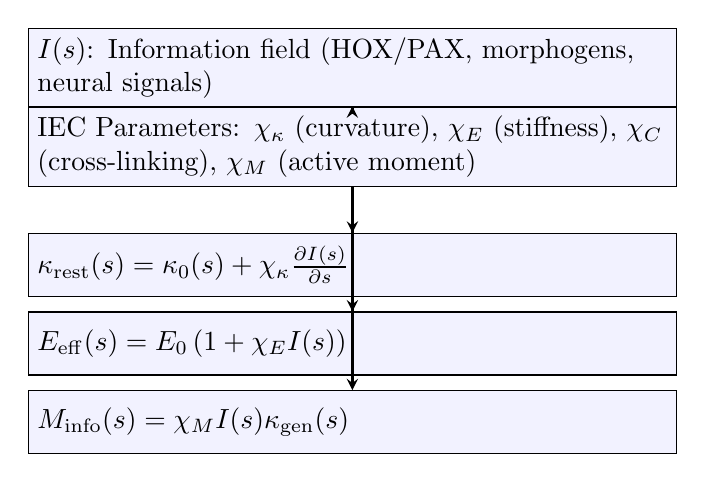
\begin{tikzpicture}[
    node distance=1cm,
    eqbox/.style={rectangle, draw, fill=blue!5, text width=8cm, minimum height=0.8cm, align=left},
    arrow/.style={->, >=stealth, thick}
]

% Information Field
\node[eqbox] (I) {$I(s)$: Information field (HOX/PAX, morphogens, neural signals)};

% IEC Parameters
\node[eqbox, below of=I] (params) {IEC Parameters: $\chi_{\kappa}$ (curvature), $\chi_{E}$ (stiffness), $\chi_{C}$ (cross-linking), $\chi_{M}$ (active moment)};

% Equations
\node[eqbox, below of=params, yshift=-0.5cm] (eq1) {$\kappa_{\mathrm{rest}}(s) = \kappa_{0}(s) + \chi_{\kappa} \frac{\partial I(s)}{\partial s}$};

\node[eqbox, below of=eq1] (eq2) {$E_{\mathrm{eff}}(s) = E_{0} \left(1 + \chi_{E} I(s)\right)$};

\node[eqbox, below of=eq2] (eq3) {$M_{\mathrm{info}}(s) = \chi_{M} I(s) \kappa_{\mathrm{gen}}(s)$};

% Arrows
\draw[arrow] (I) -- (params);
\draw[arrow] (params) -- (eq1);
\draw[arrow] (params) -- (eq2);
\draw[arrow] (params) -- (eq3);

\end{tikzpicture}
\caption{Information-Elasticity Coupling (IEC) equations. The information field $I(s)$ modulates mechanical properties through dimensionless coupling parameters $\chi_{\kappa}$, $\chi_{E}$, $\chi_{C}$, and $\chi_{M}$, producing modified rest curvature, effective stiffness, and active moments.}
\label{fig:iec_equations}
\end{figure}




\begin{figure}[h!]
    \centering
    \begin{subfigure}[b]{0.48\textwidth}
        \centering
        \includegraphics[width=\textwidth]{fig_countercurvature_panelA.pdf}
        \caption{Curvature profiles $\kappa_{0}(s)$ vs $\kappa_{I}(s)$.}
    \end{subfigure}
    \hfill
    \begin{subfigure}[b]{0.48\textwidth}
        \centering
        \includegraphics[width=\textwidth]{fig_countercurvature_panelB.pdf}
        \caption{Countercurvature metric $g_{\mathrm{eff}}(s)$ and information field.}
    \end{subfigure}

    \vspace{0.5em}

    \begin{subfigure}[b]{0.48\textwidth}
        \centering
        \includegraphics[width=\textwidth]{fig_countercurvature_panelC.pdf}
        \caption{Normalized geodesic deviation $\widehat{D}_{\mathrm{geo}}$ vs $\chi_{\kappa}$.}
    \end{subfigure}
    \hfill
    \begin{subfigure}[b]{0.48\textwidth}
        \centering
        \includegraphics[width=\textwidth]{fig_countercurvature_panelD.pdf}
        \caption{Microgravity adaptation: $\widehat{D}_{\mathrm{geo}}$ vs $g$.}
    \end{subfigure}

    \caption{Information-driven countercurvature in spine-like and plant-like configurations. 
    Panel A shows the curvature profiles for passive (gravity-only) and information-coupled configurations. Panel B displays the countercurvature metric $g_{\mathrm{eff}}(s)$ along the rod axis, highlighting regions of high information processing. Panel C demonstrates how normalized geodesic deviation $\widehat{D}_{\mathrm{geo}}$ increases with information--curvature coupling strength $\chi_{\kappa}$. Panel D shows that $\widehat{D}_{\mathrm{geo}}$ persists as gravitational loading is reduced, while passive curvature energy collapses, demonstrating information-driven structure maintenance in microgravity.
    }
    \label{fig:countercurvature_main}
\end{figure}

\begin{figure}[h!]
    \centering
    \includegraphics[width=0.65\textwidth]{fig_phase_diagram_scoliosis.pdf}
    \caption{Phase diagram in $(\chi_{\kappa},g)$ showing gravity-dominated, cooperative, and information-dominated regimes. Contours: $\widehat{D}_{\mathrm{geo}}$. Markers: points where a small thoracic asymmetry ($\varepsilon_{\mathrm{asym}}=0.05$) produces a scoliosis-like branch (high $S_{\mathrm{lat}}$ and Cobb-like angles). The scoliotic regime (shaded) emerges in the information-dominated corner where $\widehat{D}_{\mathrm{geo}}>0.3$ and small asymmetries are predicted to be amplified.}
    \label{fig:phase_diagram}
\end{figure}

\bibliographystyle{unsrtnat}
\bibliography{refs}

\end{document}
